\documentclass{article}
\usepackage{enumitem}
\usepackage{verbatim}
\usepackage{graphicx}
\usepackage{amsfonts,amsmath}
\usepackage{subcaption}
\captionsetup{compatibility=false}
\usepackage{tikz}
\usepackage{amsthm}
\usepackage{authblk,fullpage}
\usepackage[colorlinks]{hyperref}
\usepackage[capitalize]{cleveref}
\definecolor{pinegreen}{rgb}{0.0, 0.47, 0.44}
\hypersetup{citecolor=pinegreen}
\setlist[enumerate]{itemsep=0pt,topsep=1pt}
\setlist[itemize]{itemsep=0pt,topsep=1pt}


\usetikzlibrary{automata,positioning, arrows}
\newcommand{\mayqed}{}
\usepackage[algo2e, noline, boxed]{algorithm2e}
   \renewcommand{\CommentSty}[1]{\textnormal{#1}\unskip}\SetKwComment{tcm}{\{}{\}}
    \newenvironment{myfunction}[2][htbp]
   {\setlength{\algomargin}{.2cm}
     \begin{center}
     \begin{minipage}{#2}
     \begin{function}[#1]
     \small
      \let\Par=\par
        \def\par{\endgraf\vspace{.1cm}}
            \SetKw{To}{to}\SetKw{Downto}{downto}\SetKw{Or}{or}\SetKwFor{Algo}{Function}{}{}\vspace{.15cm}}
    {\let\par=\Par\end{function}\end{minipage}\end{center}}
   \newenvironment{myalgorithm}[2][htbp]
   {\setlength{\algomargin}{.2cm}
     \begin{center}
     \begin{minipage}{#2}
     \begin{algorithm2e}[#1]
     \small
      \let\Par=\par
        \def\par{\endgraf\vspace{.1cm}}
            \SetKw{To}{to}\SetKw{Downto}{downto}\SetKw{Or}{or}\SetKwFor{Algo}{Algorithm}{}{}\vspace{.15cm}}
    {\let\par=\Par\end{algorithm2e}\end{minipage}\end{center}}

  \newcommand{\defproblem}[2]{
  \noindent\begin{center}\fbox{
  \begin{minipage}{0.5\textwidth}
  \vspace{0.1cm}
  #1

  \vspace{0.2cm}
  \noindent
  #2
  \vspace{0.1cm}
  \end{minipage}
  }
  \end{center}
  \vspace{2mm}
}

   \pagestyle{plain}
   
   \newcommand{\Oh}{\mathcal{O}}
   \newcommand{\argmax}{\mathrm{arg max}}
   \newcommand{\floor}[1]{\left\lfloor #1 \right\rfloor}
   \newcommand{\ceil}[1]{\left\lceil #1 \right\rceil}
   \newcommand{\poly}{\mathit{poly}}
   \def\dotdot{\mathinner{\ldotp\ldotp}}
   \newcommand{\integ}{\mathbb{Z}}
   \newcommand{\eps}{\varepsilon}
   \newcommand{\sub}{\subseteq}
   \newcommand{\dB}{dB}
   \newcommand{\occ}{\mbox{\it occ-pos}}

   \renewcommand{\L}{{\mathcal{L}}}
   \newcommand{\CS}{\mbox{\large{\sf{S}}}}
   \newcommand{\Lynd}{\mathit{LynRank}}
   \newcommand{\rot}{\mathit{rot}}
   \newcommand{\minrot}[1]{\left\langle #1 \right\rangle}
   
   \newtheorem{theorem}{Theorem}
   \newtheorem{corollary}[theorem]{Corollary}
   \newtheorem{proposition}[theorem]{Proposition}
   \newtheorem{lemma}[theorem]{Lemma}
   \newtheorem{observation}[theorem]{Observation}
   \newtheorem{fact}[theorem]{Fact}
   \theoremstyle{definition}   
   \theoremstyle{remark}
   \newtheorem{example}[theorem]{Example}
   \newtheorem*{claim}{Claim}

   
   

\author{Tomasz Kociumaka}
\author{Jakub Radoszewski}
\author{Wojciech Rytter}

\affil{Institute of Informatics, University of Warsaw, Poland}
\affil[]{\texttt{[kociumaka,jrad,rytter]@mimuw.edu.pl}}

\date{\vspace{-1cm}}

\title{
Efficient Ranking of Lyndon Words and\\ Decoding
Lexicographically Minimal de Bruijn Sequence\footnote{
This is an extended version of our previous conference paper \cite{DBLP:conf/cpm/KociumakaRR14} with complexities reduced
by a  factor in case of the word RAM model.
}
   }

\begin{document}
\maketitle
\begin{abstract}
We give efficient algorithms for ranking Lyndon words of length  over
an alphabet of size . The rank of a Lyndon word is its position
in the sequence of lexicographically ordered Lyndon words of the same length.
The outputs are integers of exponential size, and
complexity of arithmetic operations on such large integers cannot be ignored.
Our model of computations is the word RAM, in which  basic arithmetic operations on
(large) numbers of size at most  take  time.
Our algorithm for ranking Lyndon words makes  arithmetic operations
(this would imply directly cubic time on word RAM).
However, using an algebraic approach we
are able to reduce the total time complexity on word RAM to .
We also present an -time algorithm that generates the Lyndon
word of a given length and rank in lexicographic order.
Finally we use the connections between Lyndon words and lexicographically minimal de Bruijn sequences
(a theorem of Fredricksen and Maiorana) to develop the first polynomial-time algorithm
for decoding minimal de Bruijn sequence of any rank 
(it determines the position of a given word of length  within the de Bruijn sequence).
\end{abstract}


\section{Introduction}
We consider finite words over an ordered alphabet  of size .
A \emph{Lyndon word}~\cite{Lyndon1954,chen1958free} over  is a word that is strictly smaller in the lexicographic order than all its
nontrivial cyclic rotations.
For example, for  where , the word \texttt{aababb} is a Lyndon word,
as it is smaller than its cyclic rotations: \texttt{ababba}, \texttt{babbaa}, \texttt{abbaab},
\texttt{bbaaba}, \texttt{baabab}.
On the other hand, the word \texttt{abaab} is not a Lyndon word, since its cyclic rotation \texttt{aabab}
is smaller than it.
Also the word \texttt{aabaab} is not a Lyndon word, as its cyclic rotation by 3 letters is equal to it.
Lyndon words have a number of combinatorial properties (see, e.g., \cite{Lothaire}) including the famous Lyndon
factorization theorem~\cite{chen1958free}, which states that every word can be uniquely written
as a concatenation of a lexicographically non-increasing sequence of Lyndon words

(due to this theorem, Lyndon words are also called prime words; see~\cite{Knuth}).
They are also related to \emph{necklaces} of  beads in  colors, that is, equivalence classes of -ary
-tuples under rotation~\cite{FK,fredricksen1978necklaces}.
In particular, a necklace can be identified with the lexicographically minimal tuple in its class, 
and thus it is often defined as a word of length  over alphabet of size  that is smaller than or equal to all its cyclic rotations
(or equivalently, as a power of a Lyndon word of a length that divides ).
Lyndon words and necklaces have numerous applications in the field of text algorithms;
see e.g.\ \cite{DBLP:conf/dlt/BonomoMRRS13,ApplicationsOfRuns,TextAlgorithms,DBLP:conf/soda/Mucha13}.

A \emph{de Bruijn sequence of rank }~\cite{deBruijn} is a cyclic sequence of length 
in which every possible word of length  occurs as a factor exactly once.
For example, for  the following two sequences of length 16 are de Bruijn
sequences of rank 4:

De Bruijn sequences are present in a variety of contexts, such as digital fault testing,
pseudo-random number generation, and modern public-key cryptographic schemes.
There are numerous algorithms for generating such sequences and their generalizations
to other combinatorial structures have been investigated; see~\cite{deBruijnAnalogs,Knuth}.
Fredricksen and Maiorana \cite{DBLP:journals/jct/Fredricksen70,fredricksen1978necklaces} have shown a surprising
deep connection between de Bruijn sequences and Lyndon words:
the lexicographically minimal de Bruijn sequence over  is a concatenation,
in the lexicographic order, of all Lyndon words over  whose length is a divisor of .
For example, for  and the binary alphabet we have the following decomposition of the minimal
de Bruijn sequence into Lyndon words:


\paragraph{\bf Problem definitions and previous results.}
We denote by  and  the set of all Lyndon words and
all Lyndon words of length , respectively, and define

The problem of ranking Lyndon words can be defined as follows.

\defproblem{\textbf{Problem 1.} Ranking Lyndon words}{Given a Lyndon word , compute .}

\begin{example}
  For  we have  since there are 8 Lyndon words of length 6
  that are not greater than :
  
\end{example}

What was previously known is that all Lyndon words of length at most  can be generated in lexicographic order.
The first solution is due to Fredricksen, Kessler, and Maiorana (FKM) \cite{FK,fredricksen1978necklaces};
later Duval developed an alternative algorithm~\cite{DBLP:journals/tcs/Duval88}.
The analysis by Ruskey et al.~\cite{DBLP:journals/jal/RuskeySW92} shows that the FKM
algorithm generates the subsequent Lyndon words in constant amortized time; Berstel and Pocchiola~\cite{DBLP:journals/tcs/BerstelP94} achieved an analogous result for Duval's algorithm.
A different constant-amortized-time solution, based on recursion, was given by Cattell et al.~\cite{DBLP:journals/jal/CattellRSSM00}.
However, there was no polynomial-time algorithm to generate a Lyndon word of an arbitrary rank
or for ranking Lyndon words.
Ruskey stated finding such an algorithm as a research problem in his book~\cite{RuskeyCombGen}.

An intimately related task, of ranking and unranking \emph{necklaces}, was explicitly stated as open by Martínez and Molinero~\cite{Martinez2004}.
As far as obtaining polynomial-time solutions is concerned, one can easily show equivalence of this problem with its counterpart for Lyndon words. 
Listing necklaces  also resembles listing Lyndon words: two of the previously mentioned algorithms (FKM and Cattell et al.'s) 
can be used for both tasks. Variants of the listing problem have also been considered, e.g., generating binary necklaces with a given number of zeroes and ones~\cite{DBLP:journals/siamcomp/RuskeyS99}.

Let .
By  we denote the lexicographically first de Bruijn sequence of rank  over the given alphabet .
It is the concatenation of all Lyndon words in  in lexicographic order~\cite{DBLP:journals/jct/Fredricksen70,fredricksen1978necklaces}.
For a word  of length  over , by  we denote the (1-based) position of its occurrence in .
The problem of decoding the minimal de Bruijn sequence can be stated as follows.

\defproblem{\textbf{Problem 2.} Decoding minimal de Bruijn sequence}{Given a word  over , compute .}

\begin{example}
  For  we have .
  For this sequence:
  
\end{example}

For several types of de Bruijn sequences, there exist polynomial-time decoding algorithms \cite{DBLP:journals/tit/MitchellEP96,DBLP:journals/dm/Tuliani01}.
They find the position of an arbitrary word of length  in a specific de Bruijn sequence,
which proves useful in certain types of position sensing applications of de Bruijn sequences (see~\cite{DBLP:journals/dm/Tuliani01}).
Nevertheless, no polynomial-time decoding algorithm for lexicographically minimal de Bruijn sequence was known prior to our contribution.
Note that the FKM algorithm can be used to compute the subsequent symbols of the lexicographically minimal
de Bruijn sequence with worst-case  delay~\cite{FK} and amortized  delay~\cite{DBLP:journals/jal/RuskeySW92}.
Alternative solutions achieve ~\cite{DBLP:journals/jct/Fredricksen72,DBLP:journals/jal/Ralston81} or even ~\cite{JRmgr} worst-case delay.
All these solutions only allow to generate characters of  \emph{in order}, though.

\paragraph{\bf Our model of computations.}
Our algorithms work in the \emph{word RAM} model; see \cite{DBLP:conf/stacs/Hagerup98}.
In this model, we assume that  and  fit in a single machine word;
in other words, a single machine word has at least  bits and simple arithmetic operations on
small numbers (i.e., numbers which fit in a constant number of machine words) are performed in constant time.
Basic arithmetic operations (addition, subtraction, multiplication by a small number) on numbers of size at most  take  time.

Another model of computation is the \emph{unit-cost RAM}, where each arithmetic operation
takes constant time. This model is rather unrealistic if we deal with large numbers.
However, it is a useful intermediate abstraction.

\paragraph{\bf Our results.}
We present an -time solution for finding the rank of a Lyndon word
(Problem~1).
The algorithm actually computes  for arbitrary  that are not necessarily Lyndon words.
Using binary search, it yields an -time algorithm for computing
the -th Lyndon word of length  (in the lexicographic order) for a given .
Next, we show an -time solution for decoding minimal de Bruijn sequence  (Problem~2).
We also develop an -time algorithm computing the -th symbol of
 for a given .
Additionally, we obtain analogous results for a variant  of the minimal de Bruijn sequence, introduced by Au~\cite{DBLP:journals/dm/Au15},
in which all factors of length  are primitive and every primitive word of length  occurs exactly once.
All these algorithms work in the word RAM model.
In the unit-cost RAM, the time complexities reduce by a factor of .

\paragraph{\bf Related work.}
A preliminary version of this paper
appeared as \cite{DBLP:conf/cpm/KociumakaRR14}.
At about the same time, similar results were published by Kopparty, Kumar, and Saks \cite{DBLP:conf/icalp/KoppartyKS14}.
The work in these two papers was done independently.
The papers provide polynomial-time algorithms for ranking Lyndon words and necklaces, respectively,
and these two problems can be easily reduced  to each other.
The authors in \cite{DBLP:conf/icalp/KoppartyKS14}
put the results in a broader context and have some additional applications
(indexing irreducible polynomials and explicit constructions of certain algebraic objects).
On the other hand, we exercised more care in designing the algorithm to obtain a better polynomial running time.
In particular, \cite{DBLP:conf/cpm/KociumakaRR14} contained an -time
algorithm for ranking Lyndon words in the word RAM model,
which works in  time in the unit-cost RAM.
We also obtained a cleaner approach to alphabets of size more than 2.
An alternative -time algorithm in the unit-cost RAM model was later designed by Sawada and Williams~\cite{DBLP:journals/jda/SawadaW17}.

\paragraph{\bf Structure of the paper.}
\Cref{sec:prelim,sec:comb,sec:auto,sec:arith} (and \ref{sec:debruijn}) contain a full version of the paper \cite{DBLP:conf/cpm/KociumakaRR14}.
\Cref{sec:prelim} defines the notions of self-minimal words (necklaces) and Lyndon words and lists a number of their properties.
In \cref{sec:comb} we use combinatorial tools to obtain a formula for  in the case that  is self-minimal.
The next three sections are devoted to efficient computation of the main ingredient of this formula.
In \cref{sec:auto} we show that it is sufficient to count specific walks in an auxiliary automaton.
Then in \cref{sec:arith,sec:wordram} we show efficient implementations of this technique under unit-cost RAM
and word RAM models, respectively.
In \cref{sec:debruijn}, we apply ranking of Lyndon words to obtain efficient decoding of minimal de Bruijn sequence.


\section{Preliminaries}\label{sec:prelim}
Let  be an ordered alphabet of size .
By  and , we denote the set of all finite words over  and the set of all such words of length~.
The empty word is denoted as .
If  is a word, then  denotes its length,  its -th letter
(for ),  its factor 
and  its prefix .
A suffix of  is a word of the form .
A prefix or a suffix is called proper if it is shorter than .
By  we denote a concatenation of  copies of .
Any two words can be compared in the lexicographic order:
 is smaller than  if  is a proper prefix of  or if the letter following the longest common prefix
of  and  in  is smaller than in .

By  let us denote a \emph{cyclic rotation} of 
obtained by moving  first letters of  to its end (preserving the order of the letters).
We say that the words  and  are \emph{cyclically equivalent}
(sometimes called \emph{conjugates}).
By  we denote the lexicographically minimal cyclic rotation of .
A word  is called \emph{self-minimal} (alternatively, a \emph{necklace}) if .
The following fact gives a simple property of self-minimal words.

\begin{fact}\label{fct:lynd}
  If  is self-minimal and , then
  .
\end{fact}
\begin{proof}
  Assume to the contrary that .
  Let  be the index of the first letter where these two words differ.
  Then of course .
  Let  be an integer defined as .
  Then .
  Hence, , a contradiction.
\mayqed\end{proof}



In the ranking algorithms that we design below, we make an assumption that
the input word is self-minimal.
Consequently, we often need to replace a given arbitrary word  with
the lexicographically largest self-minimal word  (of the same length) not exceeding .
In the construction of this routine, we use the following auxiliary facts.

\begin{fact}[see \cite{DBLP:journals/jal/Duval83}]\label{fct:minrot}
  For a given word , the lexicographically minimal cyclic rotation of  () and the lexicographically minimal suffix of  can be computed in  time.
\end{fact}

  \begin{fact}\label{fct:prvaux}
    Let  and , , be words of length  with the longest common prefix of length .
    If  is self-minimal and  for each , then  is self-minimal.
  \end{fact}
  \begin{proof}
    First, note that  where .
    Indeed, if , then we would have  by self-minimality of .
    However, this contradicts .
    Now, observe that  implies  and consequently  for .
    Thus,  is trivially self-minimal.
    Hence, from now on we may assume that .

    Since  for , this means that  for .
    Thus, it suffices to show that  for .
    For a proof by contradiction, suppose that . Consequently,
    
    since for  we have  with the longest common prefix of length exactly .
    However, the obtained sequence of inequalities proves that  and 
    have a common prefix of length at least  due to such a common prefix of  and .
    The contradiction concludes the proof.
  \mayqed\end{proof}

We are now ready to implement the announced procedure.

\begin{lemma}\label{lem:prv}
  For a given word  we can compute in  time the
  lexicographically largest self-minimal word  such that .
\end{lemma}
\begin{proof}
  \Cref{fct:minrot} lets us check whether  is self-minimal. If so, we simply return .
  Consequently, we may assume that the sought word  is strictly smaller than .
  Assume the longest common prefix of  and  
  is  for some .
  Then , so
  in particular  and one can choose 
  as the letter preceding . Additionally, let .
  Consider a word 
  Note that .
  If , then \cref{fct:prvaux} applied for  and 
  would show that , and this would contradict the definition of .
  Hence, .
    
  Consequently, it suffices to consider  and,
  for each  such that ,
  a word  where  is the letter preceding  in .
  Since  is guaranteed to be one of the considered words,
  it suffices to output the largest of these candidates for which .
  This procedure can be implemented in  time using \cref{fct:minrot}.
\mayqed\end{proof}

The shortest word  such that  for some positive integer  is called the
\emph{primitive root} of . We say that  is \emph{primitive} if its primitive root is  itself.
Otherwise,  is called non-primitive.
The primitive root of a word of length  can be computed in  time 
using the failure function from the algorithm of Knuth, Morris, and Pratt~\cite{DBLP:journals/siamcomp/KnuthMP77};
see~\cite{AlgorithmsOnStrings}.

We say that  is a \emph{Lyndon word} if it is primitive and self-minimal.
Equivalent definitions are that a Lyndon word is (strictly) smaller than all its suffixes or all its cyclic rotations.
All cyclic rotations of a Lyndon word are different primitive words.
Moreover, every self-minimal word can be expressed in a unique way as 
for some Lyndon word ; see \cite{Lothaire}.
Below we show an additional property of Lyndon words that will be useful in \cref{sec:debruijn}.

\begin{fact}\label{fct:lyndon}
  Let .
  \begin{enumerate}[label={(\alph*)}]
    \item\label{aa}
      It is not possible that .
    \item\label{bb}
      If , then .
  \end{enumerate}
\end{fact}
\begin{proof}
  \ref{aa} The inequalities imply that  is a proper prefix of .
  Let , where  is an integer and  is not a prefix of .
  We have
  
  If , then we conclude that .
  Otherwise, , where  and .
  Hence, , so again .
  In both cases we have , which contradicts
  the fact that a Lyndon word is smaller than all its suffixes.

  \ref{bb} Suppose to the contrary that  but .
  Then
  
  This contradicts part \ref{aa}.
\mayqed\end{proof}





\section{Combinatorics of Ranking Lyndon Words}\label{sec:comb}
Recall that, for a word , we defined  as the number of Lyndon words
in  not exceeding .
Our basic goal (stated as Problem~1) is to efficiently compute  for a given word .
It suffices to compute  for a self-minimal word .
If  is not self-minimal, then  where  is the greatest self-minimal
word such that ; such  can be computed efficiently using \cref{lem:prv}.

We will show how to reduce computation of  to the computation 
of the cardinality of the following set:

for some prefixes  of .


\begin{example}
  For ,
  there are seven words of length four lexicographically smaller than or equal to :
  
  This set contains words from the following four equivalence classes.
  Each class includes a self-minimal word that is underlined.
    
  Thus,  consists of four full classes of cyclic equivalence:
  
\end{example}

Let us introduce the following auxiliary sets defined for  and divisors :


\begin{example}
  For  and , we have
  
\end{example}

As shown in the following two facts,  is closely related to ,
which can be expressed in terms of  for .

\begin{fact}\label{fct:lyndtocsprime}
For every word , we have .
 \end{fact}
  \begin{proof}
    Observe that  is the set of all primitive words of length  that have a cyclic
    rotation not exceeding . Each Lyndon word of length  not exceeding  
    corresponds to  such words: all its cyclic rotations.
  \mayqed\end{proof}

\begin{fact}\label{fct:csprimetocs}
For every word , if , then .
\end{fact}
\begin{proof}
    We first show that
    
    For a word  of length  there exists exactly one primitive word  such that  where .
    Thus:
    
    and the sum is disjoint.
    Now  implies \eqref{eq:CS_CS1}.
    From this formula, we obtain the claimed equality by the Möbius inversion formula.
\end{proof}

The  sets are closely related to the regular  sets for prefixes  of .
It is most evident for a self-minimal word.

\begin{fact}\label{fct:C1_C}
  If  is self-minimal and , then .
\end{fact}
\begin{proof}
  If , the equality of the two sets is trivial. Assume .
  Let us prove the equality by showing both inclusions.

  Assume that .
  This means that , therefore  (as ).
  Hence, .

  Now assume that .
  This means that .
  We have
  
  where the second inequality is due to \cref{fct:lynd}.
  Hence, .
\mayqed\end{proof}

The facts that we have just proved let us derive a formula for .

\begin{lemma}\label{lem:formula}
  If a word  is self-minimal, then
  
\end{lemma}
\begin{proof}
We use Facts \ref{fct:lyndtocsprime}, \ref{fct:csprimetocs}, and \ref{fct:C1_C} in a series of transformations to express
 using ,  for , and finally  for :

\mayqed\end{proof}

\begin{example}
  Let . We have   and 
  
  
  The set of Lyndon words of length  that are not greater than  is:
  
  Indeed, it contains eight elements.
\end{example}

The next three sections are devoted to a proof of the following lemma.

\begin{lemma}\label{lem:csgen}
  For a self-minimal word , one can compute :
  \begin{enumerate}[label={(\alph*)}]
    \item\label{aaa} in  time in the unit-cost RAM,
    \item\label{bbb} in  time in the word RAM.
  \end{enumerate}
\end{lemma}

\noindent
As a consequence of this lemma, we obtain efficient ranking of Lyndon words.

\begin{fact}\label{fct:div}
  If  is a real constant,
  then .
\end{fact}
\begin{proof}
  Recall that for  we have . Consequently,
  

\vspace*{-1.1cm}\mayqed\end{proof}

\begin{theorem}\label{thm:lynd}
  For an arbitrary word  of length , one can compute   in  time in the word RAM or
  in  time in the unit-cost RAM.
\end{theorem}
\begin{proof}
  We use the formula given by \cref{lem:formula} and the algorithm of \cref{lem:csgen}.
  If any of the words ,  is not self-minimal, then instead we take the greatest word of the same length that is
  not greater than it and is self-minimal (using \cref{lem:prv}).
  The time complexity is  in the word RAM
  or  in the unit-cost RAM which, by \cref{fct:div}, reduces to  in the word RAM
  or  in the unit-cost RAM, respectively.
\mayqed\end{proof}

We also obtain an efficient algorithm for ``unranking'' Lyndon words.

\begin{theorem}\label{thm:kth}
  The -th Lyndon word of length  can be found in  time in the word RAM
  or  time in the unit-cost RAM.
\end{theorem}
\begin{proof}
  By definition of the  function, we are looking for the smallest   such that .
  We binary search  with respect to the lexicographic order, using the algorithm of \cref{thm:lynd}
  to check whether .
  The size of the search space is ,  which gives an additional -time factor.
\mayqed\end{proof}









\section{Automata-Theoretic Interpretation}\label{sec:auto}
From now on we assume that  is self-minimal.
Our goal is to compute .

\newcommand{\Pref}{\mathrm{Pref}}
Let .
Consider a language  containing words that have a factor .
Equivalently,  if there exists a factor of  which is smaller than or equal to ,
but is not a proper prefix of .
For a language , let .
\begin{fact}\label{fct:char}
  .
\end{fact}
\begin{proof}
  Consider a word . 
  If , then .
  Take , which is a factor of .
  Some prefix of  belongs to .
  This prefix is a factor of , so .
  Consequently, .

  On the other hand, assume that , so  contains a factor .
  Let us fix the first occurrence of  in . Observe that  can be extended to a cyclic rotation  of .
  Note that  implies that ,
  hence  and .
\mayqed\end{proof}

\noindent
We construct a deterministic finite automaton  recognizing .
It has  states: one for each prefix of .
The initial state is  and the only accepting state (the only element of the set ) is .
The transitions are defined as follows: we set  for any  and 

\Cref{fig:automaton} contains an example of such an automaton.

\begin{figure}[htbp]
\begin{center}
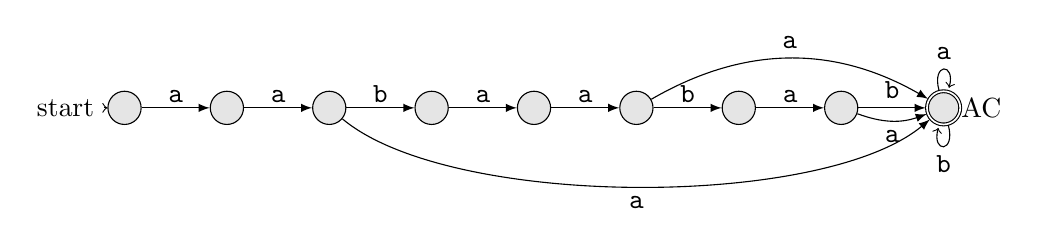
\begin{tikzpicture}[scale=.1,-latex,node distance=1.3,on grid,auto] 

  \tikzstyle{every state}=[fill=black!10,draw=black, inner sep = 0, inner sep=0, minimum size = 12]

\node[initial,state] (w0) {};
\node[state] (w1) [right =of w0] {};
\node[state] (w2) [right = of w1] {};
\node[state] (w3) [right = of w2] {};
\node[state] (w4) [right = of w3] {};
\node[state] (w5) [right = of w4] {};
\node[state] (w6) [right = of w5] {};
\node[state] (w7) [right = of w6] {};
\node[state, accepting] (AC) [right = of w7] {};
\draw (AC) node[right=0.1cm] {AC};

\path (w0) edge node[above=-.05] {\texttt{a}} (w1);
\path (w1) edge node[above=-.05] {\texttt{a}} (w2);
\path (w2) edge node[above=-.05] {\texttt{b}} (w3);
\path (w3) edge node[above=-.05] {\texttt{a}} (w4);
\path (w4) edge node[above=-.05] {\texttt{a}} (w5);
\path (w5) edge node[above=-.05] {\texttt{b}} (w6);
\path (w6) edge node[above=-.05] {\texttt{a}} (w7);
\path (w7) edge node {\texttt{b}} (AC);
\path (w7) edge [bend right=20] node[below] {\texttt{a}} (AC);
\path (AC) edge [loop above] node {\texttt{a}} (AC);
\path (AC) edge [loop below] node {\texttt{b}} (AC);
\path[draw =black] (w2) .. controls ([{shift=(-40:20)}]w2) and ([{shift=(220:20)}]AC) .. node[below] {\texttt{a}} (AC);
\path (w5) edge [bend left] node {\texttt{a}} (AC);
 
\end{tikzpicture}
 \caption{\label{fig:automaton}
   Automaton  that accepts 
   for a word  and alphabet .
   Missing links lead to the initial state.
}
\end{center}
\end{figure}
 
Note that all accepting paths in the automaton have a simple structure.
Each of them can be divided into fragments, each of which is a path that starts in ,
visits a number of states corresponding to subsequent prefixes of  and eventually goes either back to  or to .
In the latter case the word spelled by the path fragment is an element of .
After the path reaches , it stays there.
Hence, if a word  is accepted by the automaton, then it contains a factor from , so .
Consequently, .
By a more thorough analysis we show below that .
\begin{lemma}
  Let  and let  be the state of  after reading .
  If , then . Otherwise,  corresponds to the longest prefix of 
  which is a suffix of .
\end{lemma}
\begin{proof}
  The proof goes by induction on .
  If , the statement is clear.
  Consider a word  of length . Let  where .
  If , then clearly . By inductive assumption after reading  the automaton
  is in , and  is constructed so that it stays in  once it gets there.
  Thus, the conclusion holds in this case.
  From now on we assume that .

  Let  be the state of  after reading . If , clearly 
  (), and the automaton proceeds to  as desired.
  Similarly, it behaves correctly if  and .
  Consequently, we may assume that  and that  is not a suffix of .

  Take any  such that  is a suffix of  (possibly empty).
  Note that then  is a suffix of . 
  Consequently,  is a cyclic rotation of ,
  so
  
  Hence, .
  This implies that 
  could be a prefix of  only if .
  In particular,  indeed shifts to the longest prefix of  being a suffix of .
  Now we only need to prove that .
  For a proof by contradiction, choose a factor  of  such that  and  is minimal.
  Note that  is a suffix of  (since ). We have  for some 
  and . As we have already noticed, such a word cannot be a suffix of .
\mayqed\end{proof}

We say that an automaton with the set of states  is \emph{sparse}
if the underlying directed graph has  edges counting parallel edges as one.
Note that the transitions from any state  of  lead to at most 3 different
states, so  is sparse.

The following corollary summarizes the construction of .
\begin{corollary}\label{cor:auto}
  Let  be a self-minimal word. One can construct a sparse 
  automaton  with  states recognizing .
\end{corollary}

Let us use the natural extension of the transition function of an automaton into words:

For states  let us define the set 
of the labels of walks from  to .
The following lemma shows a crucial property of the words  from the language 
such that .
It makes use of the special structure of the automaton .

\begin{lemma}\label{lem:comb_crucial}
  Let . If  but ,
  then there is a unique decomposition  such that ,  and
  . 
\end{lemma}
\begin{proof}
  Let  (for ) be the shortest prefix of  which belongs to .
  Let  be the state of  after reading . 
  Also, let  be the prefix of  of length . 
  The structure of the automaton implies that  and that
   is actually the longest prefix of  which belongs to .
  Note that  and , so  implies .
  We set the decomposition so that  and .
  Uniqueness follows from deterministic behaviour of the automaton.
\mayqed\end{proof}

\begin{example}
  Let .
  Recall that the automaton  such that  was shown in \cref{fig:automaton}.
  Consider a word  of the same length as .
  For this word  and .
  Black circles below represent the states of the automaton  after processing the subsequent letters of :
  
  \begin{center}
    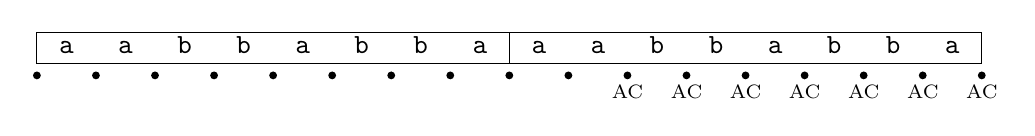
\begin{tikzpicture}[scale=1,xscale=1.5]

\foreach \x/\c in {
  0.5/a, 1/a, 1.5/b, 2/b, 2.5/a, 3/b, 3.5/b, 4/a
}{
  \draw (\x,-.4) node[above] {\tt \c};
  \draw[xshift=4cm] (\x,-.4) node[above] {\tt \c};
}

\draw[xshift=0.25cm,yshift=-0.2cm] (0,-.2) rectangle (4,.2);
\draw[xshift=4.25cm,yshift=-0.2cm] (0,-.2) rectangle (4,.2);

\begin{scope}[xshift=0.25cm,yshift=0.2cm]
\foreach \x in {0,1,...,16} {
\node[fill=black, circle, inner sep = 1] (q\x) at (\x/2 , -.75) {};
}

\draw (q0) node[below] {\footnotesize{}};
\draw (q1) node[below] {\footnotesize{}};
\draw (q2) node[below] {\footnotesize{}};
\draw (q3) node[below] {\footnotesize{}};
\draw (q4) node[below] {\footnotesize{}};
\draw (q5) node[below] {\footnotesize{}};
\draw (q6) node[below] {\footnotesize{}};
\draw (q7) node[below] {\footnotesize{}};
\draw (q8) node[below] {\footnotesize{}};
\draw (q9) node[below] {\footnotesize{}};
\draw (q10) node[below] {\scriptsize{AC}};
\draw (q11) node[below] {\scriptsize{AC}};
\draw (q12) node[below] {\scriptsize{AC}};
\draw (q13) node[below] {\scriptsize{AC}};
\draw (q14) node[below] {\scriptsize{AC}};
\draw (q15) node[below] {\scriptsize{AC}};
\draw (q16) node[below] {\scriptsize{AC}};
\end{scope}

\end{tikzpicture}
   \end{center}

  For this word the decomposition of \cref{lem:comb_crucial} is as follows:

  \begin{center}
    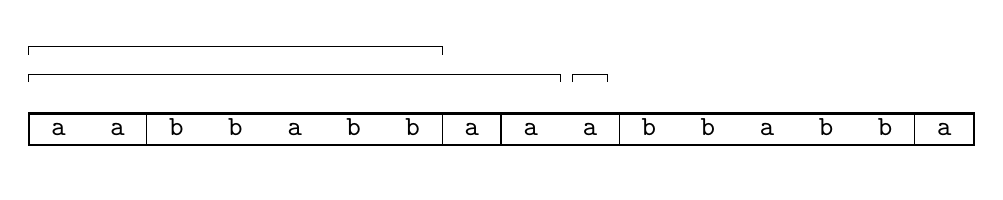
\begin{tikzpicture}[scale=1,xscale=1.5]

\foreach \x/\c in {
  0.5/a, 1/a, 1.5/b, 2/b, 2.5/a, 3/b, 3.5/b, 4/a
}{
  \draw (\x,-.4) node[above] {\tt \c};
  \draw[xshift=4cm] (\x,-.4) node[above] {\tt \c};
}

\draw[xshift=0.25cm,yshift=-0.2cm,thick] (0,-.2) rectangle (4,.2);
\draw[xshift=4.25cm,yshift=-0.2cm,thick] (0,-.2) rectangle (4,.2);
\draw[xshift=0.25cm,yshift=-0.2cm] (1,-.2) -- (1,.2)  (3.5,-.2) -- (3.5,.2);
\draw[xshift=4.25cm,yshift=-0.2cm] (1,-.2) -- (1,.2)  (3.5,-.2) -- (3.5,.2);

\begin{scope}[yshift=-0.5cm]
\draw[xshift=0.25cm] (0.5,0) node[below] {};
\draw[xshift=0.25cm] (2.25,0) node[below] {};
\draw[xshift=0.25cm] (3.75,0) node[below] {};
\end{scope}

\begin{scope}[xshift=4cm,yshift=-0.5cm]
\draw[xshift=0.25cm] (0.5,0) node[below] {};
\draw[xshift=0.25cm] (2.25,0) node[below] {};
\draw[xshift=0.25cm] (3.75,0) node[below] {};
\end{scope}

\begin{scope}[xshift=0.25cm]
\draw[yshift=0.15cm] (0,.6) -- (0,.7) -- node[above]{} (3.5,.7) -- (3.5,.6);
\draw[yshift=0.1cm] (0,.3) -- (0,.4) -- (4.5,.4) -- (4.5,.3);
\draw[yshift=0.1cm] (4,.4) node[above]{};
\draw[yshift=0.1cm] (4.6,.3) -- (4.6,.4) -- node[above] {} (4.9,.4) -- (4.9,.3);
\end{scope}

\end{tikzpicture}
   \end{center}

  In this case in the proof of the lemma we have ,
  , and .
\end{example}

Denote .
We say that a number is {\em small} if it fits into a constant number of machine words or,
in other words, is polynomial with respect to .
Using \cref{lem:comb_crucial}, we obtain a formula for .

\begin{lemma}\label{lem:cs}
  For every self-minimal word , there exist coefficients  that are small numbers such that
  
  Moreover, the coefficients  can all be computed in  time.
\end{lemma}
\begin{proof}
  We apply \cref{fct:char} with \cref{cor:auto} and actually compute
  .
  If , then obviously .
  For this part, we need to compute , which is exactly .
  Now it suffices to count  such that  but .

  Let us recall the characterization of such words from \cref{lem:comb_crucial}.
  We consider all  choices of  and ,
  and count the number of 's conditioned on these values.
  Let  where , .
  Note that , so  is a prefix  of 
  and .
  Hence,  is uniquely determined by  and .
  In particular,  and  are uniquely determined.
  Let us define  as ;
see \cref{fig:proof}.
  To efficiently determine  for each choice of  and , we precompute  for all factors  of .
  Since  these values can be computed in  time for each ,
  i.e.,  time in total.

\begin{figure}[htpb]
\centering{
  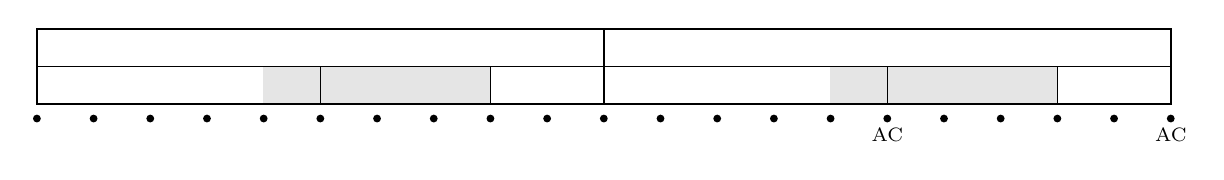
\begin{tikzpicture}[scale=1.2,xscale=1.2]

\draw (0,-.2) rectangle (5,.2);
\draw (2.5, 0) node{};
\draw (5,-.2) rectangle (10,.2);
\draw (7.5, 0) node{};
\draw (1.25, -.4) node{};
\filldraw[black!10] (2,-.2) rectangle (4, -.6);
\draw (0,-.2) rectangle (2.5, -.6);
\draw (2.5,-.2) rectangle (4, -.6);
\draw (2.25, -.4) node{};
\draw (3.25, -.4) node{};
\filldraw[black!10] (7,-.2) rectangle (9, -.6);
\draw (4,-.2) rectangle (5, -.6);
\draw (4.5, -.4) node{};
\draw (5,-.2) rectangle (7.5, -.6);
\draw (6.25, -.4) node{};
\draw (7.5,-.2) rectangle (9, -.6);
\draw (7.25, -.4) node{};
\draw (9,-.2) rectangle (10, -.6);
\draw (8.25, -.4) node{};
\draw (9.5, -.4) node{};

\foreach \x in {0,1,...,20} {
\node[fill=black, circle, inner sep = 1] (q\x) at (\x/2 , -.75) {};
}

\draw[thick] (0,-.6) rectangle (10,.2);
\draw[thick] (5,-.6) -- (5,.2);

\draw (q20) node[below] {\scriptsize{AC}};
\draw (q15) node[below] {\scriptsize{AC}};
\draw (q14) node[below] {\footnotesize{}};
\draw (q8) node[below] {\footnotesize{}};
\draw (q9) node[below] {\footnotesize{}};
\draw (q4) node[below] {\footnotesize{}};
\draw (q0) node[below] {\footnotesize{}};

\draw (17.5/2, -.9) node[below] {};
\draw (11.5/2, -.9) node[below] {};

\end{tikzpicture}
 }
\caption{\label{fig:proof}
  Illustration of \cref{lem:cs}.
  Both lines represent different factorizations of the same word .
  Black circles represent states of the automaton.
  Only shaded letters are not necessarily uniquely determined by  and  for a fixed .
}
\end{figure}
  
  Once we know , we need to count
  
  Note that , since  would
  imply that .
  Thus, the number of words  is equal to
  
  Each coefficient  can be computed in constant time, since in our automaton 
  the transition function  has an especially simple form.
  By rearranging the summands of \eqref{eq:gamma}, we obtain a formula for 
  in the desired form.
\mayqed\end{proof}







\section{Ranking Lyndon Words with  Arithmetic Operations}\label{sec:arith}
In this section by arithmetic operations we mean addition, subtraction and multiplication.
The following lemma shows how to efficiently count certain walks in the automaton  recognizing .
Its proof is based on vector-matrix multiplication.
\begin{lemma}\label{lem:mat}
  Let  be a sparse deterministic automaton with  states.
  Given  and  , it takes  arithmetic operations on integers of magnitude  to compute
  all values  and  for , .
\end{lemma}
\begin{proof}
  We construct an  matrix  with rows and columns indexed by states from .
  Set .
  It is easy to see that .
  Consequently, the entries of  belong to .
  
  Note that the matrix  is sparse, i.e., it contains  non-zero entries.
  Thus, for a (vertical) vector  one can compute  and  using  
  arithmetic operations.
  For  let  be the unit vector with one at the position corresponding to .
  Observe that  is equal to the -th entry of .
  For a fixed state , we can compute these (horizontal) vectors for  using
   vector-matrix multiplications.
  Symmetrically,  is the -th entry of ,
  and we can also compute these (vertical) vectors for  using
   matrix-vector multiplications.
  In total, we perform  arithmetic operations.
\mayqed\end{proof}

\noindent
The algorithm below combines the results obtained so far to provide the implementation for \cref{lem:csgen}\ref{aaa}.

\begin{proof}[Proof (of \cref{lem:csgen}\ref{aaa})]
Our algorithm is based on the formula of \cref{lem:cs},
whose proof already provides a procedure to compute the coefficients .
On the other hand, \cref{lem:mat} states that values  and  for 
can be determined using  arithmetic operations given the automaton recognizing .

\begin{myalgorithm}[H]{13 cm}
  \Algo{Computing  in  time in the unit-cost RAM model}
  {
    Construct automaton  for  \{ \cref{cor:auto} \}\\
    Compute  and  for all  \{ \cref{lem:mat} \}\\
    Compute  coefficients \{ \cref{lem:cs} \}\\
     \{ \cref{lem:cs} \}
  }
\end{myalgorithm}

Thus, our algorithm, given in pseudocode above, performs  arithmetic operations on integers of magnitude  to compute 
for a self-minimal word .
\mayqed\end{proof}

In the unit-cost RAM model of arithmetic operations, we obtain  time.
It is easy to check that all arithmetic operations performed in the algorithm above
are additions and subtractions of numbers not exceeding 
and multiplications of such numbers by small numbers.
Hence, in the word RAM model we obtain  time.
In the following section we give an algorithm working in  time in the word RAM model.







\section{Ranking Lyndon Words in  Time on Word RAM}\label{sec:wordram}
The improvement of the time complexity requires a modification of the formula
of \cref{lem:cs}, after which we perform  arithmetic operations only on small integers
and only  operations on large integers.
We also use Newton's iteration for power series inversion (\cite{Sieveking}; see also \cite[p.\ 140]{GeddesCL}):

\begin{fact}\label{fct:reciprocal}
  Let  be the time necessary to compute the inverse of a power series  of degree  modulo ,
  that is, the time to compute a power series  of degree  such that .
  Then  satisfies:
  
  where  is a constant and  is the time to multiply two polynomials of degree 
  with coefficients of magnitude not exceeding the -th coefficient of .
\end{fact}

\noindent
For an efficient implementation of \cref{fct:reciprocal}, we use an integer multiplication algorithm
designed for the word RAM model; see F\"urer~\cite{DBLP:conf/latin/Furer14a}.

\begin{lemma}\label{lem:multiply}
  Two polynomials of degree at most  with coefficients of magnitude 
  can be multiplied in  time in the word RAM model.
\end{lemma}
\begin{proof}
  Let  and  be the considered polynomials.
  We encode them as integers  and  as follows.
  Both  and  are divided into  chunks consisting of  bits each.
  The -th least significant chunk of  (respectively ) holds the -th coefficient of  (respectively )
  prepended by zeroes.
  Then the corresponding chunks of  hold the coefficients of .
  Both numbers  and  have  bits.
  Therefore, the product  can be computed in  time \cite{DBLP:conf/latin/Furer14a}.
\mayqed\end{proof}

\noindent
With the auxiliary \cref{fct:div}, we obtain the following tool.

\begin{lemma}\label{lem:generating}
  Let  and  be power series such that .
  Assume that the -th coefficient of  is of magnitude .
  If the coefficients of  can be computed in  time,
  then  can be computed in  time
  in the word RAM model.
\end{lemma}

Now we show how to use Lemma~\ref{lem:generating} to count specific paths in
the automaton  for the word .
Denote


\begin{lemma}\label{lem:T}
  All values  can be computed in  time in the word RAM model.
\end{lemma}
\begin{proof}
  Assume that for , .
  Recall that a non-empty path from  to itself in  passes through a number of consecutive states
   before it first comes back to .
  Hence,  satisfy the following recurrence:
  
  Let us set .
  Let  and  be the generating functions of  and :
  
  Note that:
  
  This concludes that we can use \cref{lem:generating} to compute  first coefficients of 
  in  time.
\mayqed\end{proof}

We extend the results of the previous lemma to compute the first term of the formula for .

\begin{lemma}\label{lem:complex}
  The value  can be computed in  time in the word RAM model.
\end{lemma}
\begin{proof}
  Note that
  
  where  is the number of paths of length  that start in , end in  and do not pass through  again.
  Denote . Note that  for  and .
  Moreover, for every ,
  
  as in the considered path we traverse some number of edges  passing through ,
  then we use an edge to the accepting state and stay in that state for the remaining  steps.

  Due to the recurrence , all values  can be computed in  time.
  By \cref{lem:T}, all values  can be computed in  time.
  Obviously .
  This concludes that we can use the algorithm of \cref{lem:multiply} to multiply
  the polynomials
  
  The coefficient of  at  is exactly the desired sum \eqref{eq:complex}.
\end{proof}

Finally, we are ready to prove \cref{lem:csgen}\ref{bbb}. To this end, we show that the remaining terms of the formula for  can be computed efficiently in the word RAM model.

\begin{proof}[Proof (of \cref{lem:csgen}\ref{bbb})]
  We provide an efficient implementation of the formula from \cref{lem:cs}.
  For the  part we use \cref{lem:complex}.
  Now we show how to transform the coefficients  to obtain an equivalent set of small coefficients  satisfying
   if and only if  or .
  We use the following claim.

  \medskip
  \begin{claim} For  and , we have
    
    Moreover,  for .
  \end{claim}

  \medskip
  The formula \eqref{rec} corresponds to traversing the first edge of the path from  to .
  We arrive at the following algorithm which reduces computation of the required sum of a quadratic number
  of large numbers to the computation of a linear combination of only
  linearly many big numbers .

  \begin{myalgorithm}[H]{9 cm}
    \Algo{Compute }
    {
    \ForEach{}{
      
    }
    \For{ {\rm\textbf{downto}} }{
      \For{ {\rm\textbf{to}} }{
        \\
        \\
        
      }
    }
    \Return{\hspace*{0.2cm}}
    }
  \end{myalgorithm}

  Denote .  By \eqref{rec} we have:
  
  Consequently, resetting  to zero and increasing the coefficients  and 
  in the inner iteration does not alter the total sum . 
  Hence, after every iteration of the inner for-loop the coefficients satisfy the following invariant:
  

  Observe that once  is reset to zero, it will not be changed anymore.
  Hence, at the end of the algorithm we have  if  and . Note that 
  for each  and  for .
  This concludes that at the end of the algorithm we have
  

  Note that each  coefficient accounts in 
  as at most .
  Hence, the sum of the resulting non-zero coefficients 
  does not exceed  times the sum of the initial values .
  At the end, we are to compute a linear combination of  with small coefficients.
  Consequently, \cref{lem:T} yields an -time algorithm on the word RAM.
\mayqed\end{proof}




\section{Decoding Minimal de Bruijn Sequence}\label{sec:debruijn}
In this section we focus on decoding lexicographically minimal de Bruijn sequence  over :
we aim at an efficient algorithm that for every  computes , that is,
the position of the sole occurrence of  in .
Recall that by  we denote the set of Lyndon words over  whose length is a divisor of .
A theorem of Fredricksen and Maiorana \cite{DBLP:journals/jct/Fredricksen70,fredricksen1978necklaces,Knuth}
states that  is a concatenation of the Lyndon words from 
in the lexicographic order.
The proof of the theorem is constructive,
i.e., for any word  of length  it shows the concatenation of
a constant number of consecutive Lyndon words from the cyclic version of the sequence  that contain .
This, together with the following lemma which relates  to , lets us compute the
exact position where  occurs in .

\begin{lemma}\label{lem:db}
  Let  and .
  Then the concatenation, in lexicographic order, of words 
  forms a prefix of  and its length, , is equal
  to .
\end{lemma}
\begin{proof}
  First note that, by \cref{fct:lyndon}\ref{bb}, the lexicographic order of elements 
  coincides with the lexicographic order of .
  This shows that the concatenation of elements of  indeed forms a prefix of .


  It remains to show that .
  For this we shall build a mapping 
  such that  and  for  if and only if .

  Let . There is a unique primitive word  and a positive integer  such that .
  We set .
  Note that  indeed belongs to .
  Moreover, to each Lyndon word
   of length  we have assigned  for each cyclic rotation  of .
  Thus .
  Also, , so  if and only if ,
  i.e., .
\mayqed\end{proof}

\begin{theorem}\label{thm:decoding}
  Given a word , the position  can be found in  time in the word RAM model or  time in the unit-cost RAM model.
\end{theorem}
\begin{proof}
  Let  be all Lyndon words in 
  (we have ).
  The proof of the theorem of Fredricksen and Maiorana \cite{fredricksen1978necklaces,Knuth}
  describes the occurrence of  in , which can be stated succinctly as follows.
  \begin{claim}[Fredricksen and Maiorana~\cite{fredricksen1978necklaces}, Knuth~\cite{Knuth}]
       Assume that , where  and .
     Denote  and .  
  \begin{enumerate}[label={(\alph*)}] 
    \item\label{it:simple} If  for , then  occurs in  at position .
    \item\label{it:b} If , then  is a factor of .
    \item\label{it:c} If  and , then  is a factor of .
    \item\label{it:d} If  and , then  is a factor of ,
    where  is the largest  such that .
  \end{enumerate}
  \end{claim}
  In case \ref{it:simple}, it is easy to locate  in .
  Further on, we consider only the cases \ref{it:b}, \ref{it:c}, and \ref{it:d}.

  Note that  can be retrieved as the primitive root of . For  we use the following characterization.
    \begin{claim}
      The Lyndon word  is the lexicographically larger among the following two strings:
    \begin{enumerate}[label={(\arabic*)}]
    \item\label{ONE} the longest proper prefix of  contained in ;
    \item\label{TWO} the primitive root of the largest self-minimal word  such that .
    \end{enumerate}
    \end{claim}
    \begin{proof}
  The definition of  yields , whereas
    \cref{fct:lyndon}\ref{aa} implies .
    This gives rise to two cases:
    If , then  is a proper prefix of .
    In this case,  must also be the lexicographically largest, i.e., longest, prefix of  that belongs to .
    This results in the string from case~\ref{ONE}.
    Otherwise, .
    By \cref{fct:lyndon}\ref{aa},  is the largest self-minimal length- word that is smaller than .
    That is,  corresponds to  from case \ref{TWO} and  is the primitive root of~.
    \end{proof}

  The string  can be computed efficiently using the above claim.
  In case \ref{ONE}, for each proper prefix of~, we can use \cref{fct:minrot} to check in  time if it is a Lyndon word; we then select the longest such prefix.
  In case \ref{TWO},  can be computed in  time using \cref{lem:prv}; as noted in \cref{sec:prelim}, the primitive root of  can be computed in  time.
  Finally, selecting the larger of the two candidates takes  time.
  Overall,  is computed in  time.

  Once we know  and , depending on the case, we need to find the successor in 
  and possibly the predecessor in  of one of them. 
  For any , the successor  in  can be generated by iterating a single step of the FKM algorithm at most
   times \cite{FK}, i.e., in  time.
  For the predecessor in , a version of the FKM algorithm that visits the Lyndon words
  in reverse lexicographic order can be used \cite{Knuth}.
  It also takes  time to find the predecessor.
  In all cases, we obtain in  time the Lyndon words whose concatenation contains .
  
  Then, we use exact pattern matching to locate  in the concatenation.
  This gives us the relative position of  in  with respect to the position of the canonical occurrence of  or  in .
  \Cref{lem:db} proves that such an occurrence of  \emph{ends} at position
  , which can be computed in  time in the word RAM model
  or  time in the unit-cost RAM model by \cref{lem:csgen}.
  Applied to  or , this concludes the proof.
\mayqed\end{proof}

\begin{example}
  Below we present the four cases of the claim in the proof of \cref{thm:decoding}
  on the sequence  over a binary alphabet (i.e., the lexicographically minimal binary de Bruijn sequence of rank 6), which has the following
  decomposition into Lyndon words :
  \begin{center}
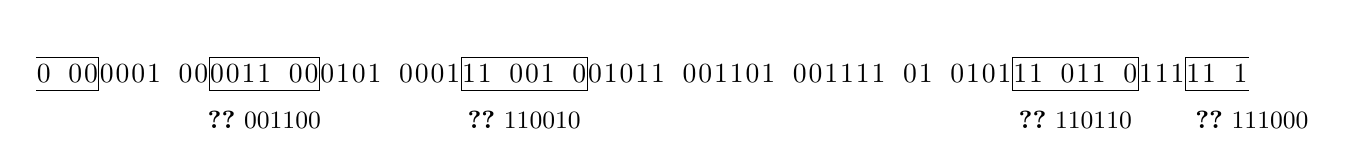
\begin{tikzpicture}[scale=0.2]

\foreach \x/\c in {
1/0,
3/0, 4/0, 5/0, 6/0, 7/0, 8/1,
10/0, 11/0, 12/0, 13/0, 14/1, 15/1,
17/0, 18/0, 19/0, 20/1, 21/0, 22/1,
24/0, 25/0, 26/0, 27/1, 28/1, 29/1,
31/0, 32/0, 33/1,
35/0, 36/0, 37/1, 38/0, 39/1, 40/1,
42/0, 43/0, 44/1, 45/1, 46/0, 47/1,
49/0, 50/0, 51/1, 52/1, 53/1, 54/1,
56/0, 57/1,
59/0, 60/1, 61/0, 62/1, 63/1, 64/1,
66/0, 67/1, 68/1,
70/0, 71/1, 72/1, 73/1, 74/1, 75/1,
77/1
}{
  \draw (\x,-.4) node[above] {\c};
}

\draw (77.5,1.8) -- (73.5,1.8) -- (73.5,-0.3) -- (77.5,-0.3);
\draw (0.5,1.8) -- (4.5,1.8) -- (4.5,-0.3) -- (0.5,-0.3);
\draw (73.5,-1) node[below right] {\small\ref{it:simple} 111000};

\draw (11.5,-0.3) rectangle (18.5,1.8);
\draw (15,-1) node[below] {\small\ref{it:b} 001100};

\draw (62.5,-0.3) rectangle (70.5,1.8);
\draw (66.5,-1) node[below] {\small\ref{it:c} 110110};

\draw (27.5,-0.3) rectangle (35.5,1.8);
\draw (31.5,-1) node[below] {\small\ref{it:d} 110010};


\foreach \x/\c in {
  1/1, 5.5/2, 12.5/3, 19.5/4, 26.5/5, 32/6, 37.5/7,
  44.5/8, 51.5/9, 56.5/10, 61.5/11, 67/12, 72.5/13, 77/14
}{
  \draw[yshift=0.5cm] (\x,2) node[above] {};
}
\end{tikzpicture}
  \end{center}
  \begin{description}
    \item{Case \ref{it:simple}:}
      , and  appears as a factor of .
    \item{Case \ref{it:b}:}
      , and  appears as a factor of .
    \item{Case \ref{it:c}:}
      , and  appears as a factor of .
    \item{Case \ref{it:d}:}
      , and  appears as a factor of .
  \end{description}
\end{example}

\medskip
\noindent
To compute the -th symbol of , we have to locate the Lyndon word from  containing
the -th position of .
We apply binary search as in \cref{thm:kth}.

\begin{theorem}\label{thm:random-access}
  Given integers  and , the -th symbol of  can be computed
  in  time in the word RAM model or  time in the unit-cost RAM model.
\end{theorem}
\begin{proof}
  We binary search for the smallest word  
  such that , using \cref{lem:csgen} to test the condition.
  In each step of the binary search, we actually consider a self-minimal word, due to \cref{lem:prv}.
  Therefore the resulting word  is of the form  for some .
  By \cref{lem:db}, a prefix of  of length  contains all Lyndon words from .
  Moreover, by \cref{fct:lyndon}\ref{aa}, this prefix ends with .
This means that the -th position of  lies within the canonical
  occurrence of . More precisely, it suffices
  to return the -th \emph{last} symbol of 
  (which is also the -th last symbol of ).
  As in \cref{thm:kth}, the binary search introduces a multiplicative
   factor to the complexity of the algorithm of \cref{lem:csgen}. 
\mayqed\end{proof}

Recently, Au \cite{DBLP:journals/dm/Au15} introduced a variant of a de Bruijn sequence
in which each (cyclic) factor of length  is primitive and each primitive word from  occurs as a (cyclic) factor.
He also proved that the lexicographically minimal sequence satisfying this condition,
denoted , is the concatenation in lexicographic order of Lyndon words of length  over .

\begin{example}
  For  and binary alphabet we have the following decomposition of :
{ 
}
\end{example}

The ranking algorithm for Lyndon words lets us derive a counterpart of \cref{thm:decoding}
for  with a slightly simpler proof (admitting a similar structure, though).
\begin{proposition}\label{prop:decoding2}
Given a primitive word , 
  can be found in  time in the word RAM model or  time in the unit-cost RAM model.
\end{proposition}
\begin{proof}
  Let  be all Lyndon words in 
  (we have ).
  The proof of a theorem of Au \cite[Theorem 9]{DBLP:journals/dm/Au15}
  describes the occurrence of  in , which can be stated succinctly as follows.
  \begin{claim}[Au \cite{DBLP:journals/dm/Au15}]
       Assume that  where  and  is a Lyndon word of length .
     Denote  and .
  \begin{enumerate}[label={(\alph*)}]
    \item\label{it:simple2} If  for , then  occurs in  at position .
    \item\label{it:b2} If , then  occurs in  at position .
    \item\label{it:d2} If , then  occurs in  at position ,
    where  is the largest Lyndon word  such that .
  \end{enumerate}
  \end{claim}

  In case \ref{it:simple2}, it is easy to locate  in  with .
  Otherwise, we observe that  and this word can be computed using \cref{fct:minrot} along with the decomposition
  .
  In case \ref{it:b2}, we observe that the position of  in 
  is , so  occurs in  at position .
  Thus, it suffices to determine  using \cref{thm:lynd}.
  The situation in case \ref{it:d2} is similar:  occurs in  at position .
  Since  is the largest Lyndon word smaller than , we have ,
  i.e., the computation is also reduced to \cref{thm:lynd}.
\end{proof}
\begin{example}
  Below we present the three cases of the claim in the proof of \cref{prop:decoding2}
  on a sequence  over a binary alphabet, which has the following
  decomposition into Lyndon words :

  \medskip
  \begin{center}
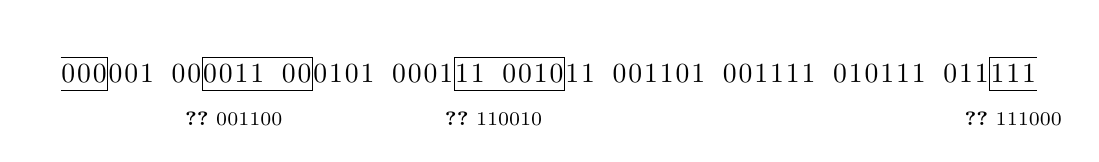
\begin{tikzpicture}[scale=0.2]

\foreach \x/\c in {
3/0, 4/0, 5/0, 6/0, 7/0, 8/1,
10/0, 11/0, 12/0, 13/0, 14/1, 15/1,
17/0, 18/0, 19/0, 20/1, 21/0, 22/1,
24/0, 25/0, 26/0, 27/1, 28/1, 29/1,
31/0, 32/0, 33/1, 34/0, 35/1, 36/1,
38/0, 39/0, 40/1, 41/1, 42/0, 43/1,
45/0, 46/0, 47/1, 48/1, 49/1, 50/1,
52/0, 53/1, 54/0, 55/1, 56/1, 57/1,
59/0, 60/1, 61/1, 62/1, 63/1, 64/1,
}{
  \draw (\x,-.4) node[above] {\c};
}

\draw (64.5,1.8) -- (61.5,1.8) -- (61.5,-0.3) -- (64.5,-0.3);
\draw (2.5,1.8) -- (5.5,1.8) -- (5.5,-0.3) -- (2.5,-0.3);
\draw (63,-1) node[below] {\scriptsize\ref{it:simple2} 111000};

\draw (11.5,-0.3) rectangle (18.5,1.8);
\draw (13.5,-1) node[below] {\scriptsize\ref{it:b2} 001100};


\draw (27.5,-0.3) rectangle (34.5,1.8);
\draw (30,-1) node[below] {\scriptsize\ref{it:d2} 110010};


\foreach \x/\c in {
  5.5/1, 12.5/2, 19.5/3, 26.5/4, 33.5/5, 40.5/6,
  47.5/7, 54.5/8,61.5/9
}{
  \draw[yshift=0.5cm] (\x,2) node[above] {};
}
\end{tikzpicture}
  \end{center}
  \begin{description}
    \item{Case \ref{it:simple2}:}
      , and  appears as a factor of .
    \item{Case \ref{it:b2}:}
      , and  appears as a factor of .
    \item{Case \ref{it:d2}:}
      , and  appears as a factor of .
  \end{description}
\end{example}

The -th symbol of  is much easier to find than the -th symbol of ,
as shown in the following result.
\begin{proposition}\label{prop:random-access2}
  Given integers  and , the -th symbol of  can be computed
  in  time in the word RAM model or  time in the unit-cost RAM model.
\end{proposition}
\begin{proof}
  The -th symbol of the sequence  is the
  -th symbol of the -th Lyndon word of length , where
  
  This word can be determined using \cref{thm:kth}.
\end{proof}





\section{Conclusions}\label{sec:concl}

The main result of this paper is an -time algorithm in the word RAM model
and an -time algorithm in the unit-cost RAM model for ranking Lyndon words.
We have also presented efficient algorithms for computing a Lyndon word of a given length and rank
in the lexicographic order, decoding lexicographically minimal de Bruijn sequence
of a given rank and computing a particular symbol of this sequence.
Our results can also be applied to ranking necklaces due to a known connection
between Lyndon words and necklaces; see \cite{DBLP:conf/icalp/KoppartyKS14}.




\section{Acknowledgements}

We would like to thank Joe Sawada for making us aware of the work of Kopparty et al.\ \cite{DBLP:conf/icalp/KoppartyKS14}.
We would also like to thank Nguyen Tien Long for spotting a minor error in the proof of \cref{thm:decoding} in a previous version of this manuscript.




\bibliographystyle{plainurl}
\bibliography{lyndon}



\end{document} 
